\documentclass[12pt]{article}
\usepackage[utf8]{inputenc}
\usepackage{graphicx}
\usepackage{float}
\usepackage{hyperref}
\hypersetup{
    colorlinks=true,
    linkcolor=blue,
    filecolor=magenta,      
    urlcolor=blue,
    pdftitle={Overleaf Example},
    pdfpagemode=FullScreen,
    }
\usepackage[export]{adjustbox}
    
\title{CS 3600 Project 3 Wrapper}
\author{CS3600 - Fall 2023}
\date{Due November 8th 2023 at 11:59pm EST via Gradescope}

\begin{document}

\maketitle

\begin{figure}[htp]
    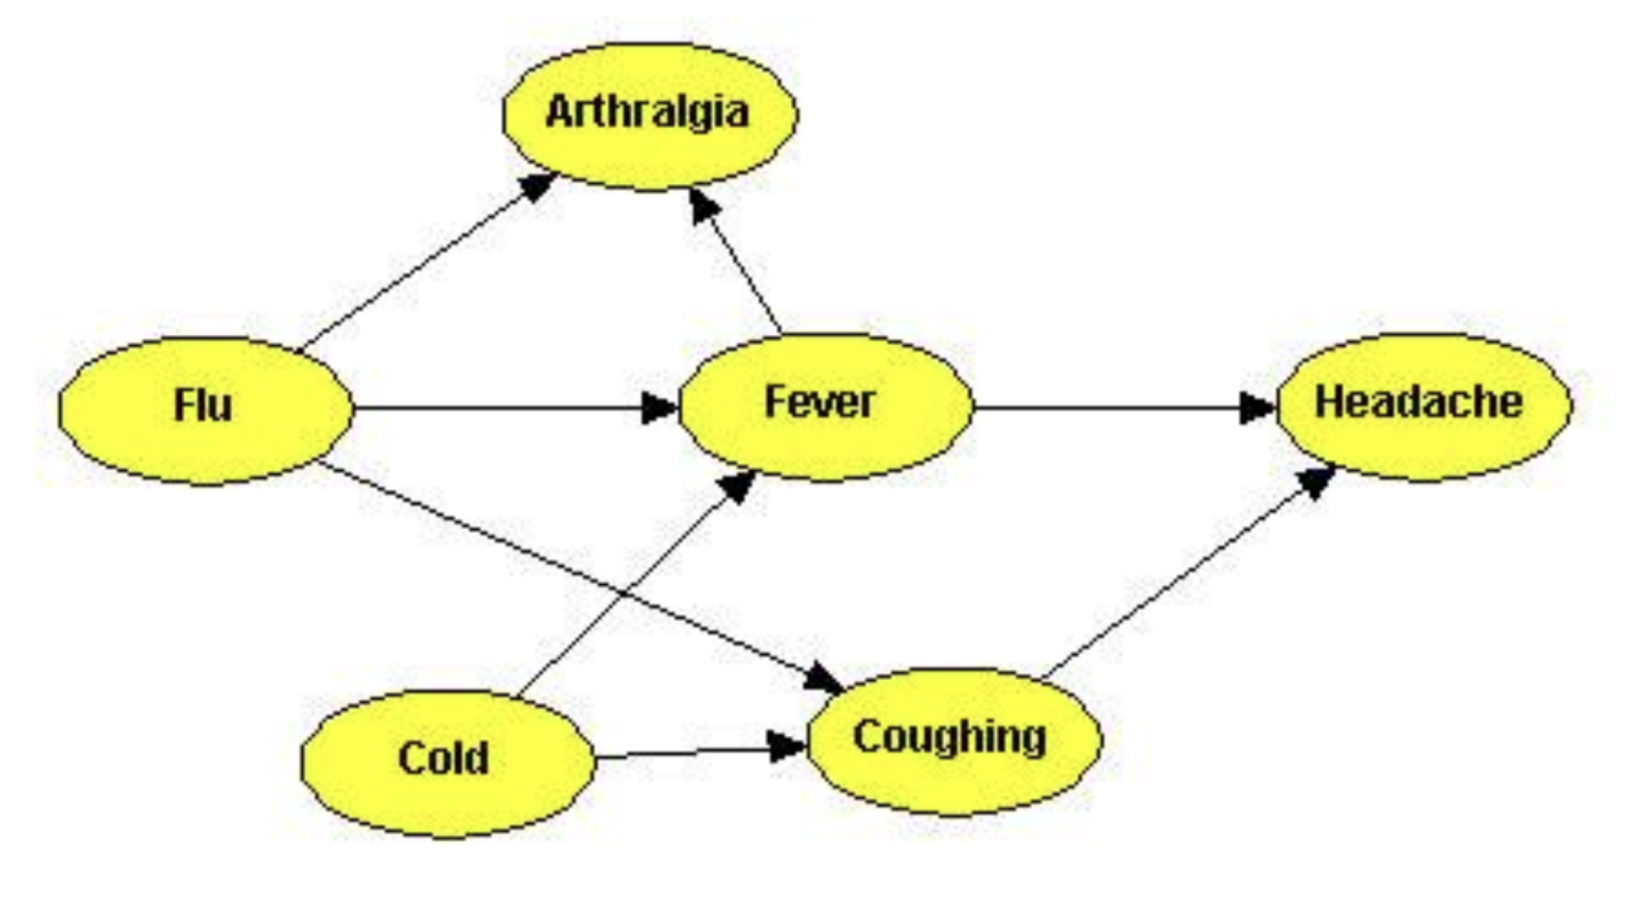
\includegraphics[width=14cm]{img/P3Q1Network.png}
    \label{fig:network}
    \caption{ Example Bayesian network for medical diagnosis. \newline Source: \url{http://song.bayesian.net/index.php/Bayesian_net}}
\end{figure}

Probabilistic inference over Bayesian networks is a standard AI technique for 
medical diagnosis. Bayesian networks represent complex causal relationships between
patient information, medical conditions, and symptoms. Probabilistic inference 
allows us to compute diagnostic queries, determining the likelihood of medical 
conditions given observed symptoms as evidence.Use the example Bayes net above as a
prompt for the following questions.
\newpage

\section*{Question 1} Recall that the naïve Bayes assumption is that no effects of a
cause are also causes of each other. If two effects are correlated it is because 
they are related to the same, underlying cause. The naïve Bayes model provides an 
alternative representation for diagnostic inference. Draw a Bayes net representing 
the naïve Bayes model for diagnosing \textit{Flu} given its symptoms (assume the 
symptoms of \textit{Flu} are every successor of \textit{Flu} in the Bayes net in 
Figure 1). Which model (the Bayes net in Figure 1 or the naïve Bayes model that 
you've constructed) is a richer representation? That is to say, is there anything 
we can represent with one model that we cannot represent with the other model? \\

\noindent\textbf{Answer:}

\newpage


\section*{Question 2}

\begin{table}[h]
    \centering
    \begin{tabular}{|c|c|c|}
    \hline
        \textbf{$SICK_{t-1}$} & $P(SICK_{t}=T | SICK_{t-1})$ & $P(SICK_t=F | SICK_{t-1})$ \\
        \hline
        T & 0.7 & 0.3 \\
        \hline
        F & 0.5 & 0.5 \\
        \hline
    \end{tabular}
    \caption{Transition Probabilities}
    \label{tab:my_label}
\end{table}
\begin{figure}[htp]
    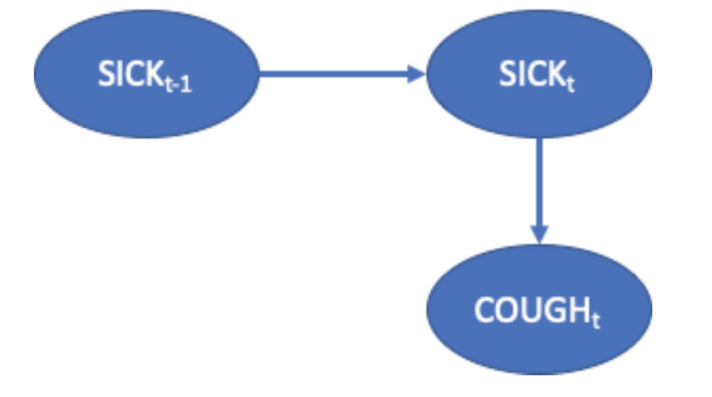
\includegraphics[width=9.5cm, center]{img/P3Q2Bayes.png}
    \label{fig:bayes}
    \caption{First Order Markov Dynamic Bayes Net}
\end{figure}
The traditional Dynamic Bayes Net has an unobservable random variable $X_t$ that 
has a single parent of the value of $X_{t-1}$, which is the value of X at the 
previous time step. For example, SICK$_t$ is conditioned on SICK$_{t-1}$. This can 
capture a relationship such as "when one is sick, the probability is high that one 
is still sick at the next time step, and when one is not sick, one can become sick 
or stay well with equal probability". See the image for an example. However, if one
were to use this Bayes network to predict the future, the model may conclude that 
people become sick randomly and then stay sick. This setup does not account for 
second-order effects, such as: "after one is sick for a while, the probability is 
high that one stops being sick". A 2-Markov assumption states that an unobservable 
random variable $X_t$ is conditioned on $X_{t-1}$ and $X_{t-2}$. \textbf{Using a
time step equal to a week, draw a 2-Markov Dynamic Bayes Network
that captures the intuition that one can become sick at any time}. When 
one is sick one is likely to remain sick unless they have been sick for two weeks, 
at which time they are likely to cease being sick. When one is sick, the 
probability of cough is high and when one is not sick, the probability of cough is 
low. \textbf{Show all the conditional probability tables; 
make up reasonable numbers to express the relationships 
described above.} \\

\noindent\textbf{Answer:}

\newpage

\section*{Question 3}
Medical diagnosis with Bayesian networks are currently used as
a \textit{decision support systems} by healthcare professionals. An expert can 
input patient information and observed symptoms, and the decision support system 
outputs a set of possible diagnoses with associated likelihoods, but the final 
diagnosis decision is up to the medical professional. Why should we require a human
supervisor to accept or override the decision of the AI diagnosis system? Name two 
(2) potential sources of error or unaccounted for situations for these Bayes net 
diagnosis models that are mitigated by having a trained healthcare professional 
make the final diagnosis decision. \\

\noindent\textbf{Answer:}

\newpage

\section*{Question 4} Publicly accessible online services often use databases and 
symptom matching to inform users of possible medical conditions given a list of 
symptoms. These services do not provide diagnosis likelihoods. Could providing a 
free online service with Bayes-net-based medical diagnosis have negative impacts on
human behavior? Could they have positive impacts? If you answered yes to either 
question, give one example. If you answered no, explain why not. \\

\noindent\textbf{Answer:}

\end{document}